To get this machinery going it is necessary to find points in the images that are interesting to look at and follow through out the sequence. It is the correspondences between points in different images that will provide the information needed to reproduce the sequence in 3D. 

\subsubsection{Feature Extractor}
The feature extraction was carried out using Harris feature detector. This method uses the local structure tensor to sort out interesting parts of the image according to \eqref{eq:Harris}. This will generate a function where the value in each point is the level if interest in that local region. To select points one can threshold this at an appropriate level and morphologically shrink it to points. Besides the level of threshold one may also be interested in the closest distance between feature points. 

To be able to estimate the fundamental matrix of an image pair it is important to have known points all over the images. It is however not necessary to have more than eight corresponding points to calculate minimal estimate the fundamental matrix, also the calculation complexity will be reduced with fewer points. This motivates the finding few, properly spread out feature points. 

\begin{equation}
\label{eq:Harris}
C_{Harris} = det(A) - \kappa \cdot trace^2(A), \hspace{1cm} \kappa \approx 0.04
\end{equation} 

\begin{equation}
\label{eq:StructureTensor}
A =  \begin{bmatrix}
	   \langle \frac{\partial I}{\partial x} \rangle^2 &  \langle \frac{\partial I}{\partial x y} \rangle \\
	   \langle \frac{\partial I}{\partial x y} \rangle & \langle \frac{\partial I}{\partial y} \rangle^2
	  \end{bmatrix}
	  , \hspace{1cm} I = image
\end{equation}

\begin{figure}[htb]
	\centering
	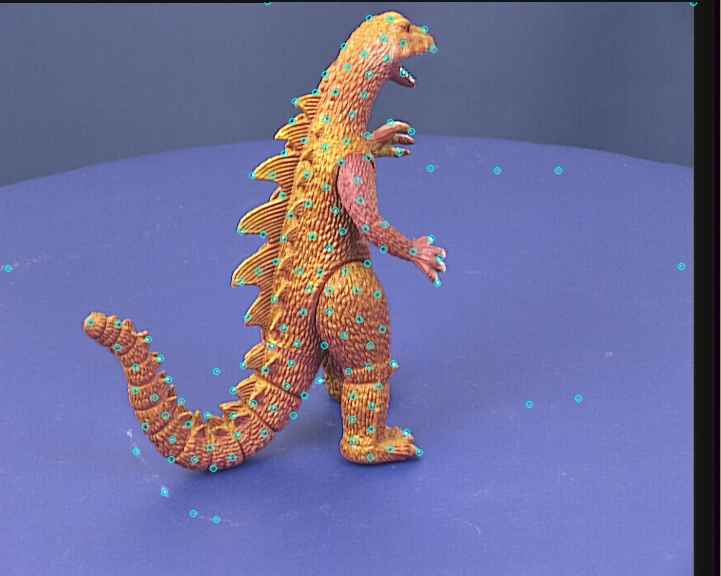
\includegraphics[width=110mm]{images/FeatureDetection.png}
	\caption{\textit{Feature points indicated with small circles. Notice the even distribution on the dinosaur body.}}
	\label{fig:FeaturePoints} %Skapar referens till figuren
\end{figure}

\subsubsection{Descriptor Extractor}
For all of the detected feature points a descriptor is calculated. This is done to be able to compare the features in different images. In this project the SIFT (Scale Invariant Feature Transform) descriptor is used. It is very effective in reducing unwanted effects of changes in illumination, scale and rotation. The way the descriptor work is that it calculates a series of histograms from magnitude and orientation values from a small region around the feature point. The histograms are stored in a high dimensional vector, that once it has been normalized is the finished SIFT descriptor.

\subsubsection{Matching}
Finally, to find the correspondences between feature points in different images, the SIFT descriptors are compared between all feature points in the images. The descriptors that are most alike are chosen as a pair. There is also a check done to see that the found match is the closest possible match. This is done to remove potential outliers. A final check to get rid of matches that still slip through the first test is done in a euclidean distance shareholding. Points are not allowed to match on a to great distance.

Later in the pipeline a RANSAC (Random Sampling Consensus) algorithm is used to remove outliers while estimating the fundamental matrix, $F$, between images. The fundamental matrix defines a necessary but not sufficient constraint for corresponding feature points called the epipolar constraint, \ref{eq:EpipolarConstraint}. If a point pair diverge to far from zero it is discarded.

\begin{equation}
\label{eq:EpipolarConstraint}
y_1^T \boldsymbol{F} y_2 = 0
\end{equation} 

\begin{figure}[htb]
	\centering
	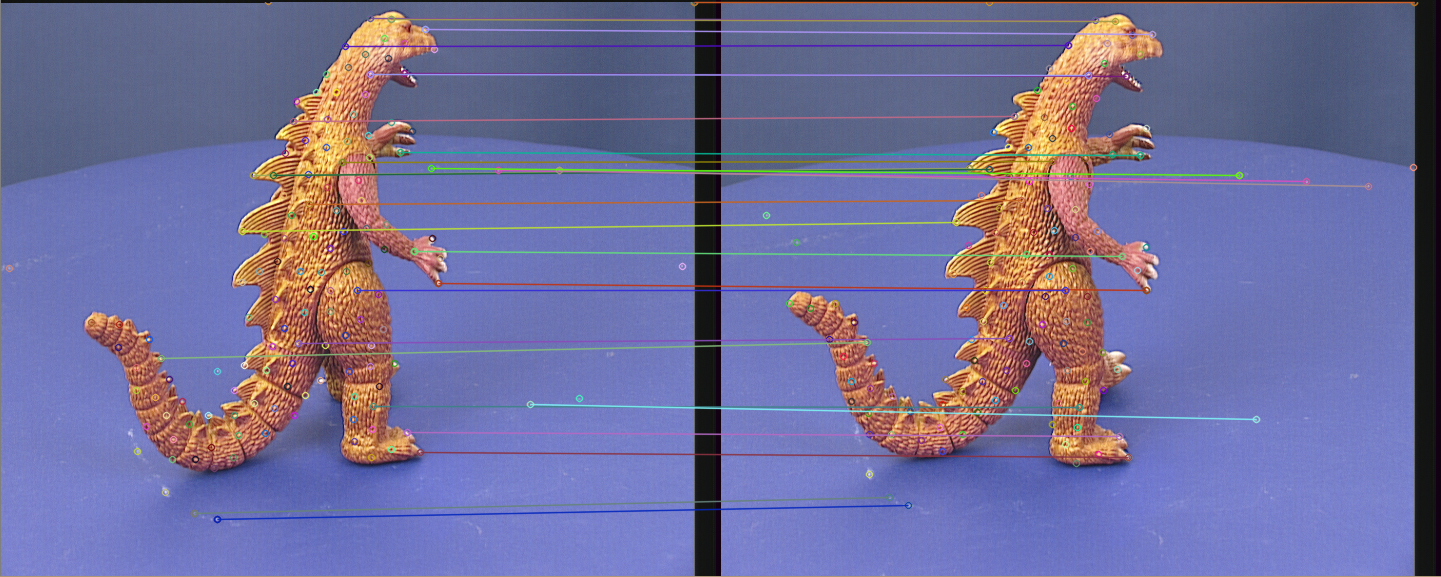
\includegraphics[width=\textwidth] {images/CorrespondenceDetection.png}
	\caption{\textit{Correspondences indicated with lines. Circles without a line attached lack correspondence.}}
	\label{fig:Correspondences} %Skapar referens till figuren
\end{figure}